\documentclass[11pt]{article}

\usepackage[utf8]{inputenc}
\usepackage[T1]{fontenc}
\usepackage{lmodern}
\usepackage[a4paper,margin=2.5cm]{geometry}
\usepackage{microtype}
\usepackage{amsmath,amssymb,amsthm}
\usepackage{graphicx}
\usepackage{booktabs}
\usepackage{enumitem}
\usepackage[font=small,labelfont=bf]{caption}
\usepackage{xcolor}
\usepackage[hidelinks]{hyperref}
\usepackage[capitalise,noabbrev]{cleveref}

\setlist{itemsep=2pt,topsep=4pt}
\setlength{\emergencystretch}{2em}
\newtheorem{theorem}{Theorem}
\newcommand{\code}[1]{\texttt{#1}}
\newcommand{\E}{\mathbb{E}}

\title{When Does Failure-Domain Metadata Help Tool-Using AI Agents?\\[4pt]
\large A Controlled Replication, a Label-Quality Condition,\\ and Two Surveys of MCP Server Metadata}
\author{Luong Tuan Kiet}
\date{Draft, October 2026}

\begin{document}
\maketitle

\begin{abstract}
Tool-using AI agents can receive outputs that are wrong yet schema-valid. When two differently named tools draw on the same upstream source, cross-verification between them only produces false agreement. Prior work shows that choosing a corroborator with a different lineage sharply reduces unsafe decisions, but it assumes that lineage labels are available and correct. We ask how accurate failure-domain metadata must be, and how accurate real metadata is.
(1) In a controlled refund-decision simulation with accurate metadata, choosing a corroborator from a different failure domain reduces unsafe decisions from 30/150 to 0/150 (95\% CI of the difference $[-0.273,-0.127]$); the advantage is not robust when 25\% of labels are wrong.
(2) We prove, under stated assumptions, that metadata-guided selection beats random selection if and only if $J = r - \varphi > 0$, and is worse when $J<0$; a preregistered test on 60 new tasks confirms both directions ($J=-0.5$: $+0.133$ $[+0.070,+0.200]$).
(3) Two surveys of open-source MCP servers (42 and 78 servers) find that 16\% and 27\% of same-type server pairs share an upstream provider. Agent-visible metadata omits the provider in about 70\% of pairs, but is mostly correct when present ($J=0.89$ with READMEs); the second survey meets 4 of 6 preregistered predictions.
The practical bottleneck is \emph{missing} metadata rather than wrong metadata. Survey labels are AI-coded without independent human validation, and no result measures live-agent behaviour.
\end{abstract}

\noindent\textbf{Keywords:} tool-using AI agents; correlated failures; common-mode failures; failure-domain metadata; provenance; Model Context Protocol; empirical survey.

%======================================================================
\section{Introduction}\label{sec:intro}

LLM agents are increasingly allowed to call APIs, read databases and take actions with real consequences, such as issuing refunds or deleting resources. Agents treat tool outputs as evidence about the outside world. The most dangerous failure is a \emph{silent tool failure}: the call succeeds and the output is schema-valid, but its content is wrong or stale.

A natural defence is \emph{cross-verification}: before acting, the agent consults a second tool (a \emph{corroborator}) and proceeds only if the two agree. The number of tools, however, is not the number of independent sources of evidence. Two differently named tools may call the same provider. When that provider is wrong, both tools are wrong in the same way, and the agent sees false agreement (\cref{fig:problem}). This is the familiar \emph{common-mode failure} of dependable systems~\cite{kl86}, and correlated errors have also been observed across LLMs~\cite{ce25}.

\begin{figure}[t]
  \centering
  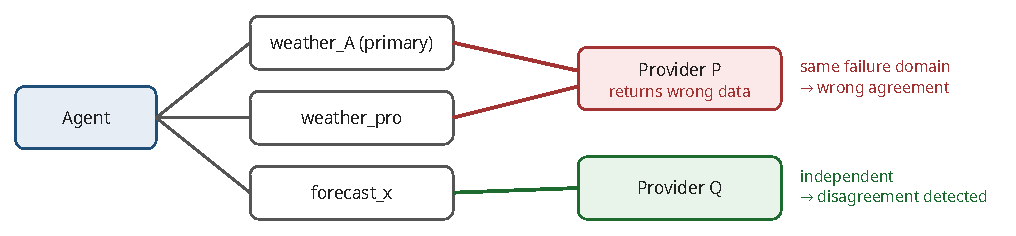
\includegraphics[width=0.85\linewidth]{figures/problem-common-mode.pdf}
  \caption{The primary \code{weather\_A} and \code{weather\_pro} have different names but call the same Provider~P, so they share a failure domain. When P returns wrong data, choosing \code{weather\_pro} as corroborator yields false agreement; \code{forecast\_x} calls an independent Provider~Q and exposes the disagreement. Illustrative example.}
  \label{fig:problem}
\end{figure}

If the agent knows which tool belongs to which failure domain, it can choose an independent corroborator. VP-Control~\cite{vpc26} measured this with a strong design (preregistration, a live study): under a common-stale regime, false approval is 91.5\% when both verifier calls share the source and 9.8\% when one uses an independent source. EFD~\cite{efd26} proves that adding reviewers cannot repair a shared upstream. Both \emph{assume that lineage labels are available and correct}. Bara~\cite{bara26} shows why this assumption matters: from report content alone one cannot distinguish independent reports from copies of the same evidence, so information about sources must come from outside. In practice that information comes from tool names, descriptions and documentation, and it can be missing or wrong.

We study this gap through three research questions:
\begin{itemize}
  \item \textbf{RQ1 (replication).} \emph{Given accurate failure-domain metadata, under targeted common-mode silent tool-output failures, does independent-domain corroboration reduce unsafe refund authorization decisions relative to random corroboration at a matched two-observation budget?} This replicates VP-Control in another domain; it is not a new finding.
  \item \textbf{RQ2 (label quality).} \emph{Under class-conditional failure-domain label errors, for which combinations of shared-dependency recall $r$ and false-sharing rate $\varphi$ does failure-domain-aware selection beat, match, or lose to random selection?}
  \item \textbf{RQ3 (real metadata).} \emph{Among open-source MCP servers that provide the same information type, how often do two servers share an upstream data provider, and how well does agent-visible metadata reveal that sharing?}
\end{itemize}

\paragraph{Contributions.} (1) A simple condition, with a proof, that tells when failure-domain metadata helps, does nothing, or harms, together with a preregistered test. (2) Empirical evidence, replicated on two samples, on the quality of real MCP server metadata, including predictions that failed. (3) A controlled replication of RQ1 with a negative robustness result and a power analysis. We propose no new algorithm and claim no superiority over prior work.

\paragraph{Chronology.} RQ2 and RQ3 were formulated \emph{after} the RQ1 results were known and after we found VP-Control. Every subsequent data collection and test followed a protocol written and confirmed in advance, and every later change was logged as a dated amendment. These protocols are internal, not registered with an independent registry.

%======================================================================
\section{Problem Formulation}

\paragraph{Failure domain.} A set of components that can fail together because of a shared dependency, such as one API provider.

\paragraph{Selectors.} An agent has a primary tool and $n$ candidate corroborators, of which $s$ truly share the primary's failure domain. Metadata labels each corroborator as \emph{shared} or \emph{independent}.
\code{random\_k} chooses uniformly among the $n$ candidates, so it picks a shared tool with probability $s/n$.
\code{provenance\_k} chooses uniformly among candidates labelled independent, and falls back to a uniform choice among all $n$ if there are none.

\paragraph{Label quality.} We treat metadata as a classifier of ``shares the primary's domain'':
the \emph{recall} $r$ is the probability that a truly shared tool is labelled shared;
the \emph{false-sharing rate} $\varphi$ is the probability that a truly independent tool is labelled shared;
and $J = r - \varphi$, analogous to Youden's index in diagnostics.

\paragraph{Survey quantities.} Over pairs of servers that provide the same information type, $\rho$ is the share of pairs that truly share a provider, and $m$ is the share of pairs with a missing label (at least one side names no provider); $r$, $\varphi$ and $J$ are computed on labelled pairs. Metadata is measured at two levels: \textbf{L1} is what an agent sees at run time (server name, tool names and descriptions, input schema), and \textbf{L2} adds the README. Sharing is defined at two levels: the \emph{operator level} (the organisation operating the API host the tool calls by default) and the \emph{data-origin level} (the ultimate data source, when evidence exists).

%======================================================================
\section{Related Work}

\paragraph{Cross-tool verification and action gating.} RIVA uses multiple diagnostic paths to improve reliability when observability tools return errors~\cite{riva26}. Deterministic pre-execution gates~\cite{rlvm26}, postcondition verification~\cite{vtc26} and pre-action verification~\cite{lbyl26} already exist. Two ProvenanceGuard systems check claim attribution~\cite{pgf26} and the grounding of tool calls~\cite{pga26}. These works do not report a controlled comparison of failure-domain-aware corroborator selection under shared-backend corruption; this is a difference in the question measured, not evidence that those methods fail.

\paragraph{Tool trust.} TEA-CXA learns query-dependent tool expertise~\cite{tea26}, and other work calibrates uncertainty in tool use~\cite{pc24}. Knowing that a tool is usually right does not tell whether two tools rarely fail together.

\paragraph{Lineage-aware verification.} VP-Control~\cite{vpc26} and EFD~\cite{efd26} are the closest prior art (\cref{sec:intro}). Work on agent dependency graphs~\cite{grade26,af26} recovers dependency structure from code, which is not ground truth for whether two backends fail together at run time.

\paragraph{MCP ecosystem.} Measurement studies report that 88.6\% of 116 official MCP servers are fully or partially backed by existing REST APIs~\cite{mcprest25}, and that MCP servers show dependency monocultures~\cite{mcpmeas25}. They do not measure whether servers providing the same information share a provider, or whether metadata reveals it.


%======================================================================
\section{RQ1: Controlled Replication}

\paragraph{Design.} We use the deterministic support-desk environment \code{trajectory-judge} (commit \code{d0ee54aa}). The primary \code{check\_eligibility} and \code{check\_eligibility\_search} share \code{operational\_db}; the other two corroborators belong to two other domains. A deterministic actor reads the primary: if eligible it proposes a refund, otherwise it escalates. Every refund proposal must pass one corroborator ($K=2$ observations); if the two agree the refund is authorized, otherwise it is escalated. The design crosses 30 tasks, 5 seeds, 3 regimes (clean, independent fault, targeted common-mode) and 3 policies, for 1,350 decision rows. The outcome is an \emph{unsafe refund decision}, scored by a code oracle rather than an LLM judge. Inference uses a paired task-cluster bootstrap (10,000 resamples). This is a decision simulation: no refund is executed and no LLM is run.

\paragraph{Results.} Under the targeted common-mode fault, \code{random\_k} makes 30/150 unsafe decisions and \code{provenance\_k} makes 0/150 (difference $-0.200$, 95\% CI $[-0.273,-0.127]$). Clean correctness is 150/150 for both. The independent-fault negative control shows no advantage ($+0.007$, $[-0.020,0.033]$). The result follows almost directly from the topology: the random selector picks the same-domain tool about one third of the time. It is \emph{containment}, not recovery: under the targeted fault both policies make 0/50 correct refund decisions, because the actor never proposes a refund after the primary's false denial.

\paragraph{Robustness to imperfect metadata.} A follow-up study used 30 new tasks and 3,750 rows (\cref{tab:robust}). The overall robustness gate \textbf{fails}, so RQ1 is restricted to accurate metadata. A post-hoc analysis predicts an effect of about $-0.088$ under wrong labels, and shows that the locked criterion had only about 56\% power at 30 tasks (83\% at 60). We keep the FAIL; it is weak evidence that the advantage disappears, not evidence that it remains. The question of how wrong labels may be before the advantage vanishes leads to RQ2.

\begin{table}[t]
\centering
\caption{Robustness of the RQ1 advantage (provenance minus random unsafe rate).}
\label{tab:robust}
\begin{tabular}{lrll}
\toprule
Condition & $\Delta$ unsafe & 95\% CI & Gate \\
\midrule
Accurate labels, leakage 0.25 & $-0.133$ & $[-0.220,-0.053]$ & PASS \\
25\% labels missing, leakage 0.10 & $-0.153$ & $[-0.227,-0.087]$ & PASS \\
25\% labels wrong, leakage 0.10 & $-0.067$ & $[-0.133,\ 0.000]$ & \textbf{FAIL} \\
\bottomrule
\end{tabular}
\end{table}

%======================================================================
\section{RQ2: The $J$ Condition}

\begin{theorem}\label{thm:j}
Assume that the primary's label is correct, that corroborator labels are mutually independent and depend only on the true class (shared or independent), and that selection is uniform with uniform fallback. Let $a = 1-r$ be the probability that a shared tool is a candidate, $b = 1-\varphi$ the probability that an independent tool is a candidate, and $K$ the number of other candidates. Then
\[
P(\text{select a shared tool}) - \frac{s}{n} \;=\; -\,\frac{s(n-s)}{n}\, J\; \E\!\left[\frac{1}{1+K}\right].
\]
\end{theorem}

Both $s(n-s)/n$ and $\E[1/(1+K)]$ are positive, so \emph{the sign of the difference is the sign of $-J$}: provenance beats random iff $J>0$, ties at $J=0$, and loses when $J<0$. \emph{Proof idea:} pair one shared tool with one independent tool; the remaining candidates have the same distribution from the viewpoint of both, so when the two selection probabilities are subtracted every term cancels except $(b-a)\,\E[1/(1+K)]$, and $b-a=J$. If each label is present only with probability $k$, then $a=k(1-r)$ and $b=k(1-\varphi)$, so $b-a=kJ$: \emph{missing labels shrink the effect but never flip its sign}. The closed form matches exact enumeration to $10^{-16}$; a numerical sweep over 2,205 grid points in 5 topologies, checked by independent Monte Carlo, shows no violation.

\paragraph{Example.} In the main topology ($n=3$, $s=1$) with $r=0$ and $\varphi=0.5$ ($J=-0.5$), provenance selects the shared tool with probability $0.583$ versus $0.333$ for random: bad metadata is worse than none.

\paragraph{Preregistered test.} To check that the condition survives the full pipeline (actor, gate, leakage, oracle) and not only the selection formula, we wrote the protocol and hypotheses in advance and ran them on 60 \emph{new} tasks with 5 new seeds, 4 label conditions and 2 policies (4,800 rows, leakage 0.10). One amendment corrected a prediction \emph{before} the run, after a unit test showed that it used a wrong assumption. \Cref{tab:jtest} and \cref{fig:j} show the results. Both main hypotheses (harm when $J<0$, benefit when $J>0$) are supported, and the differences lie close to the predictions. H-J3 (equivalence at $J=0$, margin $\pm0.08$) is \emph{not} confirmed: the 90\% CI $[+0.013,+0.117]$ exceeds the margin. Its power (about 59\%) was not planned, and we do not interpret the result as harm at $J=0$, because the protocol did not register that hypothesis.

\begin{table}[t]
\centering
\caption{Preregistered test of the $J$ condition: unsafe decision rates under the targeted fault (\checkmark{} supported, $\times$ not supported).}
\label{tab:jtest}
\small
\setlength{\tabcolsep}{3.5pt}
\begin{tabular}{lrrrrll}
\toprule
Condition & Prov. & Random & $\Delta$ & Predicted & 95\% CI & Hypothesis \\
\midrule
$J=+0.8$ ($r$ 0.9, $\varphi$ 0.1) & 0.087 & 0.263 & $-0.177$ & $-0.176$ & $[-0.233,-0.120]$ & H-J2 \checkmark \\
$J=0$ ($r$ 0.5, $\varphi$ 0.5) & 0.320 & 0.257 & $+0.063$ & $0.000$ & $[+0.003,+0.127]$ & H-J3 $\times$ \\
$J=-0.5$ ($r$ 0.1, $\varphi$ 0.6) & 0.423 & 0.290 & $+0.133$ & $+0.160$ & $[+0.070,+0.200]$ & H-J1 \checkmark \\
Survey ($r$ 0.57, $\varphi$ 0, $k$ 0.55) & 0.173 & 0.267 & $-0.093$ & $-0.091$ & $[-0.157,-0.033]$ & H-J4 \checkmark \\
\bottomrule
\end{tabular}
\end{table}

\begin{figure}[t]
  \centering
  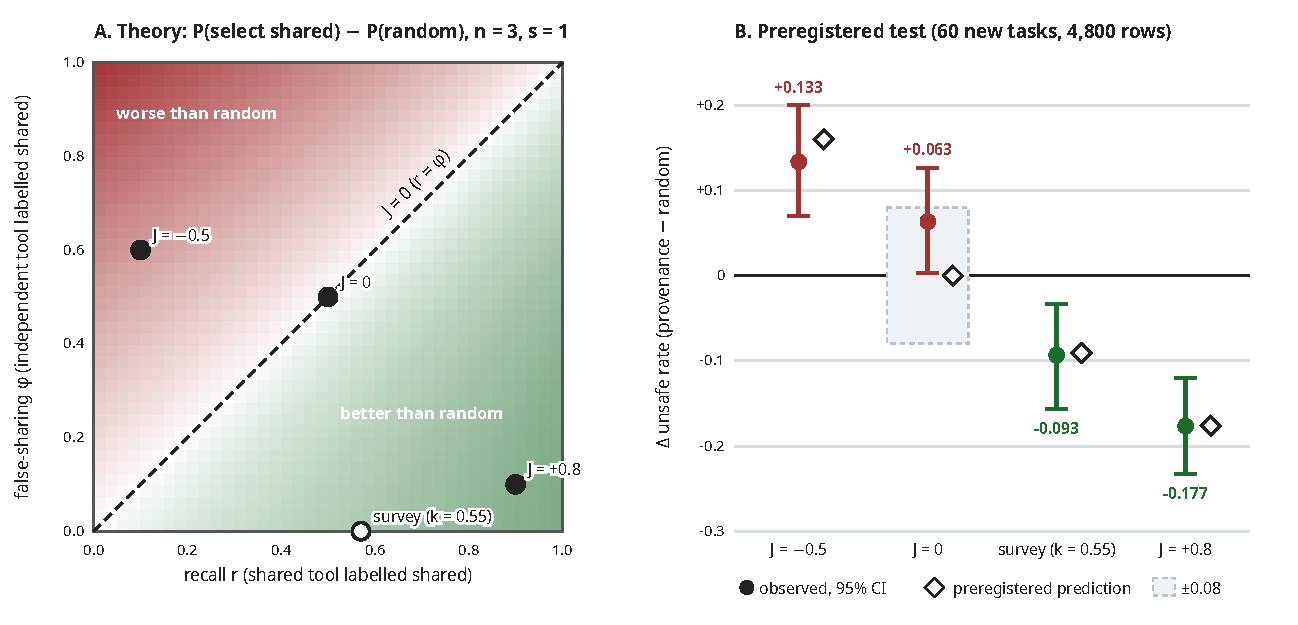
\includegraphics[width=\linewidth]{figures/rq2-j-condition.pdf}
  \caption{(A) Closed-form $P(\text{select shared}) - s/n$ for the main topology over $(r,\varphi)$: green is better than random, red is worse; the boundary is exactly the diagonal $J=0$. The hollow point (survey-calibrated) has missing labels and is shown for reference only. (B) Unsafe-rate differences in the preregistered test with 95\% CIs; diamonds are preregistered predictions; the grey band is the $\pm0.08$ equivalence margin.}
  \label{fig:j}
\end{figure}

\paragraph{Limits of RQ2.} This is a simulation we designed, so the outcome is largely implied by the model; its value lies in test discipline (predictions written in advance, new tasks), not novelty. The theorem does not cover labels correlated across tools, a wrong primary label (which is exactly the robustness-gate model of RQ1), or selection of several corroborators.

%======================================================================
\section{RQ3: Metadata of Real MCP Servers}

\subsection{Method}

We ran two surveys, each under a protocol confirmed before the sampling frame was built.
\begin{itemize}
  \item \textbf{Sampling.} For each information type, a fixed GitHub query \code{"<keyword> mcp server"} sorted by stars; the result list was locked with SHA-256 before any code was read, with predefined fallback queries for thin categories. Survey~1 covers 7 types (weather, currency exchange, stocks, crypto, geocoding, web search, news) with 6 servers each: 42 servers and 105 pairs. Survey~2 is a new sample that excludes every survey-1 repository, adds 5 types (translation, IP geolocation, movies, books, air quality) and takes 8 servers per type: 78 servers, of which 74 (245 pairs) enter pooled estimates because two types had fewer than 4 eligible servers.
  \item \textbf{Screening} in rank order against five criteria: public repository; a real Model Context Protocol implementation; a tool returning the information type; an external API call; a default upstream. Screening errors found during coding were corrected by the predefined rank-order rule (1 in survey 1, 4 in survey 2).
  \item \textbf{Ground truth.} Static reading of the code at a pinned commit, without running it, to identify the provider each tool calls by default, with \code{file:line} evidence. Two servers \emph{share} if their default provider sets intersect.
  \item \textbf{Declared metadata.} Only providers named explicitly at L1 or L2 count.
  \item \textbf{Data-origin level.} Post hoc in survey 1, \emph{preregistered} in survey 2 using only evidence inside the repositories, in two variants: a literal reading of names, and an informed reading that knows, for example, that Frankfurter distributes ECB data.
  \item \textbf{Predictions.} Six predictions P1--P6 derived from survey 1, each with a pass rule written in advance. Three amendments, each made before the affected metrics were computed: A1 clarified the codebook; A2 recorded five interpretation rules that arose during coding and the analysis implementation; A3 defined the author-adjudication procedure.
  \item \textbf{Coding.} Coder A is an AI (Claude). A second coder (a team member) independently coded 10 servers in survey 1 and 20 in survey 2, chosen by hash, but \emph{used an AI (Claude or Codex)}, contrary to the plan of a human coder. Agreement is therefore between AI coders.
\end{itemize}

\subsection{Results}

\paragraph{Survey 1} (operator level). $\rho = 17/105 = 0.16$ (server-level bootstrap 95\% CI $[0.075,0.281]$), highest for web search (0.47). L1 metadata is missing in \textbf{70\%} of pairs; where present, $r=8/8$ and $\varphi=0/24$. At L2, $m=0.05$, $r=17/17$, $\varphi=0/83$. At the data-origin level (post hoc), literal-name recall drops to 0.61 (17/28), and every web-search pair shares at least one engine.

\paragraph{Survey 2} (operator level). $\rho = 67/245 = 0.27$ $[0.179,0.374]$. $\rho$ varies widely by type: currency 0.64 (six servers use Frankfurter), web search 0.39, weather 0.36, down to translation 0.04. L1 metadata is missing in \textbf{71\%} of pairs, and in every pair for weather and stocks; where present, $r=23/27$, $\varphi=3/45$, $J=0.79$. At L2, $m=0.22$, $r=52/55$, $\varphi=7/135$, $J=0.89$ (\cref{tab:origin}).

\begin{table}[t]
\centering
\caption{Survey 2 at the operator and data-origin levels (L2 metadata).}
\label{tab:origin}
\begin{tabular}{lrllr}
\toprule
Level & $\rho$ & $r$ & $\varphi$ & $J$ \\
\midrule
Operator & 0.27 & 0.95 (52/55) & 0.05 (7/135) & 0.89 \\
Data origin, literal names & 0.31 & 0.83 (55/66) & 0.03 (4/124) & 0.80 \\
Data origin, informed & 0.31 & 0.97 (64/66) & 0.02 (2/124) & 0.95 \\
\bottomrule
\end{tabular}
\end{table}

\Cref{tab:pred} checks the preregistered predictions. Two survey-1 findings do \emph{not} replicate: that labels are never wrong when present, and that web search has no independent source. All three L1 false-sharing pairs arise because metadata names the \emph{data source behind} the API rather than its operator; for example, a server calls the Blockchain Academics API while its description says prices come ``via CoinGecko''. At the data-origin level two of these three labels are correct. This interpretation is post hoc; the primary result for P3 remains a failure.

\begin{table}[t]
\centering
\caption{Preregistered predictions of survey 2.}
\label{tab:pred}
\small
\begin{tabular}{p{5.6cm}p{3.6cm}p{4.2cm}}
\toprule
Prediction & Rule & Result \\
\midrule
P1 Sharing exists but is not common & $0.05 \le \rho \le 0.30$ & 0.27, \textbf{met} (CI upper bound 0.37) \\
P2 L1 labels are usually missing & $m_{L1} > 0.50$ & 0.71, \textbf{met} \\
P3 Present labels are rarely wrong & $\varphi_{L1} \le 0.05$ & 0.067 (3/45), \textbf{not met} \\
P4 Operator names miss origin-level dependence & $r_{\text{origin}} < r_{\text{operator}}$ (L2) & 0.83 $<$ 0.95, \textbf{met} \\
P5 Some type has no independent source & $\rho_{\text{origin}} \ge 0.80$ for some type & max 0.71 (web search), \textbf{not met} \\
P6 Real metadata has $J>0$ & $J_{\text{operator},L2} > 0$ & 0.89, \textbf{met} \\
\bottomrule
\end{tabular}
\end{table}

\begin{figure}[t]
  \centering
  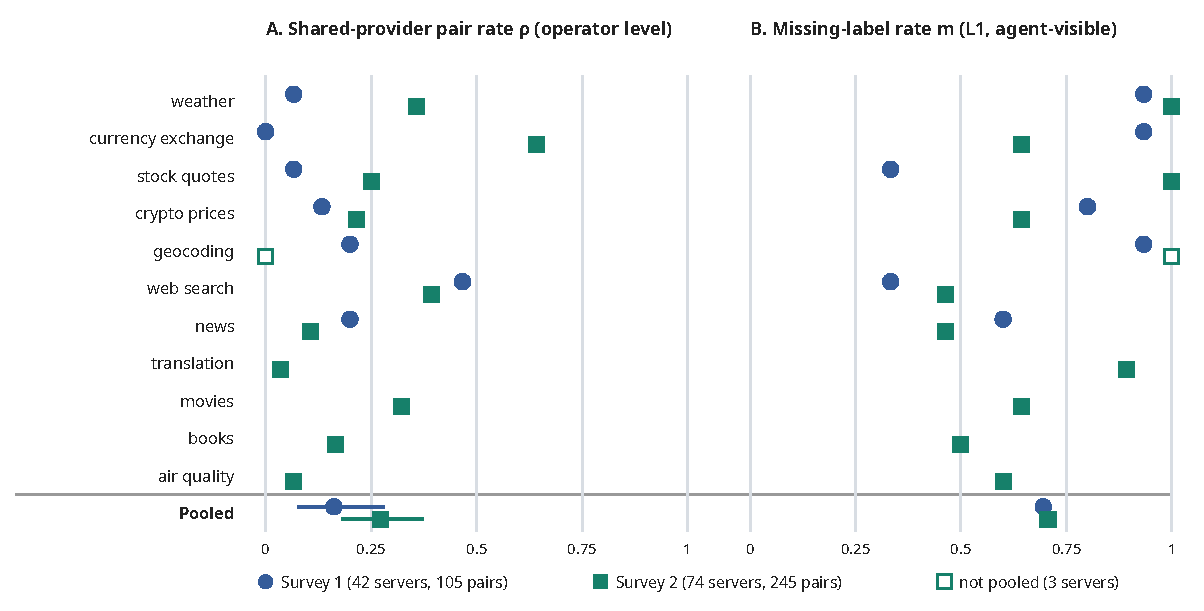
\includegraphics[width=\linewidth]{figures/rq3-surveys.pdf}
  \caption{(A) Operator-level shared-provider rate $\rho$ and (B) L1 missing-label rate $m$, by information type, for survey 1 (circles) and survey 2 (squares). The pooled row shows the 95\% bootstrap interval for $\rho$. $\rho$ for the same type changes sharply between samples, while pooled $m$ is almost unchanged (0.70 and 0.71).}
  \label{fig:surveys}
\end{figure}

\paragraph{Projection onto the selector model} (not a measurement of agents). With the label rates observed in survey 2, the probability of choosing a shared corroborator is 0.436 for random selection, 0.289 with L1 metadata, and 0.109 if README-level information were present in tool descriptions.

\subsection{Label Reliability}

\paragraph{Agreement between AI coders.} In survey 1, after name normalisation, agreement is 0.80 on upstream providers (Cohen's $\kappa=0.78$) and 1.00 on L1. In survey 2 (Claude versus Codex), with a name table fixed in advance, agreement is 0.45 on upstream ($\kappa=0.43$) and 0.65 on L1 ($\kappa=0.57$). Most disagreements are different names for the same organisation (e.g.\ \code{Google Maps Platform} versus \code{Google}); after post-hoc organisation-level merging, agreement is 0.85 on upstream and 0.80 on L1. Most importantly, whether an L1 label is present, the quantity behind the main finding, agrees on \textbf{20/20} servers ($\kappa=1.00$).

\paragraph{Author adjudication.} Lacking a human coder, the author followed a procedure recorded in the protocol before seeing the cases: he chose four codebook rules where the two AI coders diverged (e.g.\ ``the provider is the ultimate data source'' and ``providers not enabled by default do not count''), adjudicated four cases with blinded answers, and checked 10 randomly sampled \code{file:line} evidence citations, all of which were correct. Applying these rules to all 78 servers changes 7 labels. P1, P2, P4, P5 and P6 are unchanged; P3 moves from 3/45 to 2/45 $=0.044$. The false-sharing rate therefore sits \emph{at the 5\% threshold} and depends on the definition. This adjudication is not independent: the author agreed with coder A in 7 of 8 decisions, coder A also explained the questions, and the author read code lines quoted by coder A.

%======================================================================
\section{Discussion}

\paragraph{Answers.} \emph{RQ1:} with accurate metadata, choosing a corroborator from a different failure domain prevents unsafe decisions, consistent with VP-Control; the advantage is not robust to wrong labels, partly for lack of power. \emph{RQ2:} metadata helps if and only if $J>0$ and harms when $J<0$; this is proved within the model and confirmed in simulation on new tasks. \emph{RQ3:} among real MCP servers, provider sharing is real (16--27\% of pairs) and varies strongly across samples; metadata is missing in about 70\% of pairs; when present it is mostly right ($J>0$), but usually only at the operator level.

\paragraph{Implications} (inferences that need further validation).
\begin{enumerate}
  \item \textbf{The bottleneck is missing metadata, not wrong metadata.} Because $J>0$, real metadata does not harm selection under the theorem; it is simply too sparse. Moving the provider name from the README into the tool description is a cheap change that, in the projection, lowers the chance of choosing a shared corroborator from 0.289 to 0.109. This is a concrete recommendation for MCP server authors and tool registries.
  \item \textbf{Operator names are not enough.} At the data-origin level, provider names miss about 17\% (survey 2, preregistered) to 39\% (survey 1, post hoc) of dependencies; Frankfurter distributes ECB data, and differently named web-search servers call the same engines. Trustworthy registries should also publish data origins.
  \item \textbf{Independent sources can be scarce.} In web search, every surveyed server shares an engine with at least one other server. Good metadata then helps only partially, and an agent should recognise when no independent source exists and escalate, rather than treating agreement between two tools as strong evidence.
\end{enumerate}

%======================================================================
\section{Threats to Validity}

\begin{itemize}
  \item \textbf{Chronology.} RQ2 and RQ3 were posed after the RQ1 results; the initial RQ2 analysis was post hoc. Later protocols were written in advance but are internal.
  \item \textbf{Simulation.} RQ1 and the preregistered test are decision simulations designed by us; their outcomes are close to by-construction and yield no live-agent effect estimate. A small diagnostic with a real agent (Qwen2.5 7B) did not meet the condition for estimating an effect.
  \item \textbf{Independent corroborators are assumed truthful} apart from leakage. VP-Control reports that on FinQA small verifiers misread evidence and the source effect reverses; an independent source helps only if the verifier is competent.
  \item \textbf{Scope of the theorem.} It does not cover correlated labels, a wrong primary label, or multiple corroborators, and the proof has not been checked independently.
  \item \textbf{Survey labels.} They are AI-coded and the second coder also used AI. Agreement between AI coders shows that labels are reproducible, not that they are correct. The only human checks are the author's adjudication and the 10 evidence citations. The five survey-2 interpretation rules were set by coder A after reading code but before computing metrics.
  \item \textbf{Construct of sharing.} The operator level is a lower bound on true dependence; the non-empty-intersection rule overstates dependence for multi-source aggregators; the data-origin level uses only in-repository evidence.
  \item \textbf{Sample.} Popular GitHub MCP repositories only; pairs are not independent because each server appears in several pairs; the denominators of L1 recall are small (8 and 27); $\rho$ by type differs widely between samples.
  \item \textbf{Projections are not measurements of agents.}
\end{itemize}

%======================================================================
\section{Conclusion}

Two differently named tools can agree on the same wrong output when they share a failure domain. Choosing corroborators by failure domain helps only when metadata detects shared dependence more often than it reports false sharing ($J>0$); otherwise it is worse than choosing at random. We prove this condition within a model and confirm it with a preregistered test. Across two samples of real MCP servers, metadata is rarely wrong but often \emph{missing}, and when present it names the API operator rather than the underlying data origin. The most practical improvement is therefore not detecting wrong metadata but getting tools to \emph{publish} their providers and data origins where agents can read them.

\bibliographystyle{plain}
\bibliography{refs}

\end{document}
